% Options for packages loaded elsewhere
\PassOptionsToPackage{unicode}{hyperref}
\PassOptionsToPackage{hyphens}{url}
%
\documentclass[
  12pt,
]{article}
\usepackage{amsmath,amssymb}
\usepackage{lmodern}
\usepackage{iftex}
\ifPDFTeX
  \usepackage[T1]{fontenc}
  \usepackage[utf8]{inputenc}
  \usepackage{textcomp} % provide euro and other symbols
\else % if luatex or xetex
  \usepackage{unicode-math}
  \defaultfontfeatures{Scale=MatchLowercase}
  \defaultfontfeatures[\rmfamily]{Ligatures=TeX,Scale=1}
\fi
% Use upquote if available, for straight quotes in verbatim environments
\IfFileExists{upquote.sty}{\usepackage{upquote}}{}
\IfFileExists{microtype.sty}{% use microtype if available
  \usepackage[]{microtype}
  \UseMicrotypeSet[protrusion]{basicmath} % disable protrusion for tt fonts
}{}
\makeatletter
\@ifundefined{KOMAClassName}{% if non-KOMA class
  \IfFileExists{parskip.sty}{%
    \usepackage{parskip}
  }{% else
    \setlength{\parindent}{0pt}
    \setlength{\parskip}{6pt plus 2pt minus 1pt}}
}{% if KOMA class
  \KOMAoptions{parskip=half}}
\makeatother
\usepackage{xcolor}
\usepackage[margin=1in]{geometry}
\usepackage{graphicx}
\makeatletter
\def\maxwidth{\ifdim\Gin@nat@width>\linewidth\linewidth\else\Gin@nat@width\fi}
\def\maxheight{\ifdim\Gin@nat@height>\textheight\textheight\else\Gin@nat@height\fi}
\makeatother
% Scale images if necessary, so that they will not overflow the page
% margins by default, and it is still possible to overwrite the defaults
% using explicit options in \includegraphics[width, height, ...]{}
\setkeys{Gin}{width=\maxwidth,height=\maxheight,keepaspectratio}
% Set default figure placement to htbp
\makeatletter
\def\fps@figure{htbp}
\makeatother
\setlength{\emergencystretch}{3em} % prevent overfull lines
\providecommand{\tightlist}{%
  \setlength{\itemsep}{0pt}\setlength{\parskip}{0pt}}
\setcounter{secnumdepth}{-\maxdimen} % remove section numbering
\usepackage{float} \floatplacement{figure}{H}
\ifLuaTeX
  \usepackage{selnolig}  % disable illegal ligatures
\fi
\IfFileExists{bookmark.sty}{\usepackage{bookmark}}{\usepackage{hyperref}}
\IfFileExists{xurl.sty}{\usepackage{xurl}}{} % add URL line breaks if available
\urlstyle{same} % disable monospaced font for URLs
\hypersetup{
  pdfauthor={Fletcher Ekern},
  hidelinks,
  pdfcreator={LaTeX via pandoc}}

\title{\vspace{-3.5cm}

Blue Jays CMJ Report}
\author{Fletcher Ekern}
\date{}

\begin{document}
\maketitle

\hypertarget{purpose}{%
\subsubsection{Purpose}\label{purpose}}

The purpose of this report is to highlight jumps from the 2022 season
for 5 players within the Toronto Blue Jays organization.

\hypertarget{methods}{%
\subsubsection{Methods}\label{methods}}

Counter Movement Jump data from 5 separate players within the Toronto
Blue Jays organization was provided and processed. Trials where weight
was greater than 5 standard deviations away from that players mean were
filtered out. Body weight (BW), propulsive impulse (PI), peak propulsive
force asymmetry (PF) and workload were investigated, with comparisons
being made at the both the group and player level. Weight in kilograms
was calculated as the system weight in Newtons divided by gravity
(9.81). PI was normalized to BW by dividing PI by the players weight in
kg. Workload was monitored with a rolling 28-day z score ribbon +/- 2
standard deviations (sd) similar to statistical process control (Sands,
2017). When a date is outside of the ribbon, this is an instance where a
player is possibly in a state of detraining or overreaching, which can
lead to an increased risk of injury. PI was used as a metric because of
its correlation to jump height as well as being a time constrained
metric (Benjanuvatra, 2013). Since Hawkins Dynamic does not have a PI
asymmetry calculation PF was used as a way to show imbalances between
the left and right leg. A 10-15\% imbalance between the 2 has been shown
to have an increase risk of injury (Hewitt, 2012 and Cone, 2020). PI was
used for the workload monitoring as well because of fatigue's effect on
force production and the speed of signal transportation between the
muscles and brain.

\hypertarget{results}{%
\subsubsection{Results}\label{results}}

\hypertarget{weight}{%
\paragraph{Weight}\label{weight}}

With baseball being a long, grueling season the ability for a player to
maintain a steady weight is imperative when it comes to performance. A
large increase or decrease in weight can be red flag for possible injury
as well as for performance. Weight fluctuations may arise from
fluctuations in workload and/or poor nutrition habits (either eating too
much or too little). Figure 1 shows Player 5 did not do a great job of
maintaining weight throughout the year. Around the end of September,
this player was well above 2 sd from the group mean, and what also may
be a red flag is the quick drop of around 5 kilos (\textasciitilde10
lbs) within a month from the end of September to the end of October. The
one date that we have BW for Player 1, they are well below average and
may just be a small player in stature. Players 2, 3, and 4 seem to have
done a good job of maintaining their weight throughout the season are
around average for the group with no major fluctuations. Player 2 had a
steady decline in weight after the All-Star break, which may be a red
flag in isolation, but when taken in context of other metrics may not
be.

\begin{figure}
\centering
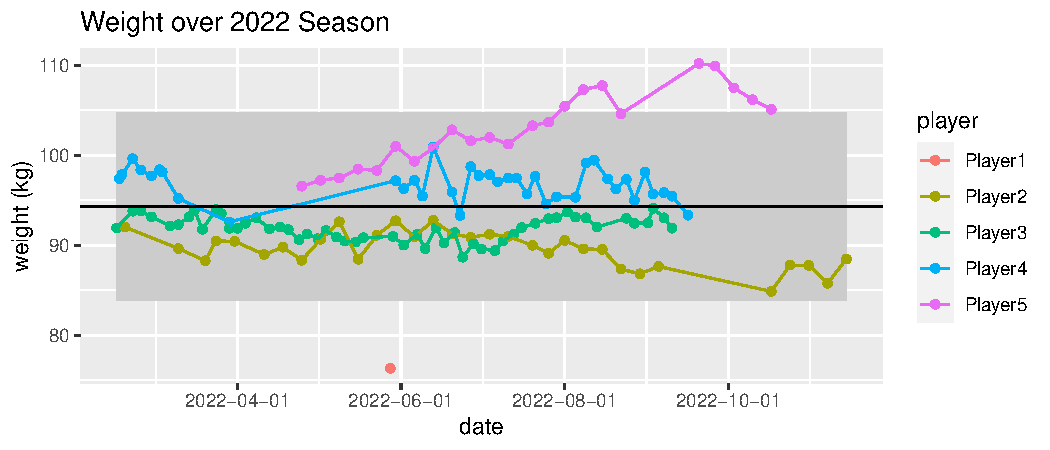
\includegraphics{report_code_files/figure-latex/weight-1.pdf}
\caption{Weight over the 2022 season by player. Black line is data set
mean. Ribbon is +/- 2 sd}
\end{figure}

\hypertarget{propulsive-impulse}{%
\paragraph{Propulsive Impulse}\label{propulsive-impulse}}

When comparing players using PI scaled to BW as the metric players 2, 3,
and 4 are all average to above average when compared to the group
(Figure 2). As noted above, Player 2's decline in BW corresponded with
increases in PI so this player has possibly improved their body
composition and is able to create force quicker at this BW. Player 5,
however is below average and drops outside of 2 sd of the group mean.
The extra weight that Player 5 put on seems to not correlate to
performance and is possibly a result of a decrease in body composition.
Player 1 has a below average PI for their BW so this player may benefit
from a general strength training and nutrition plan.

\begin{figure}
\centering
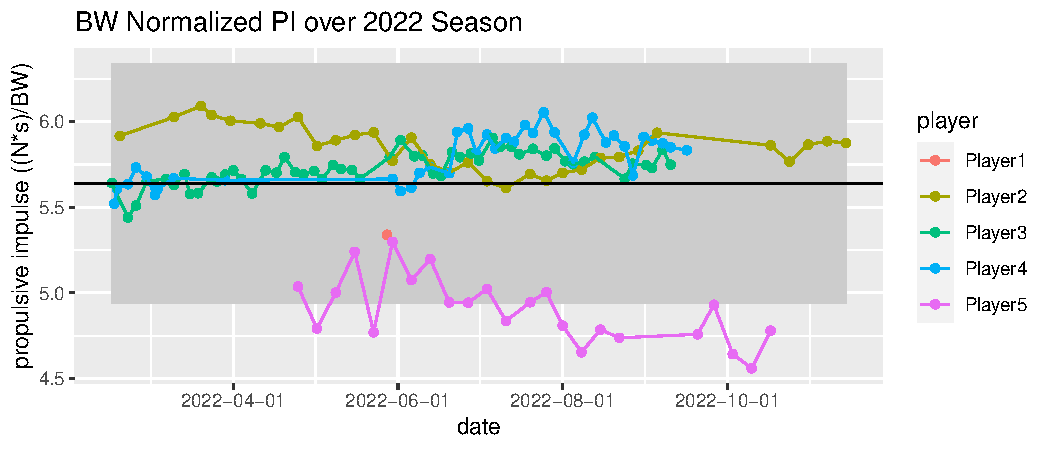
\includegraphics{report_code_files/figure-latex/propulsive impulse-1.pdf}
\caption{Propulsive impulse normalized to weight over the 2022 season by
player. Black line is data set mean. Ribbon is +/- 2 sd}
\end{figure}

\hypertarget{asymmetry}{%
\paragraph{Asymmetry}\label{asymmetry}}

All players were able to stay within the 10\% difference threshold.
Player 3 developed a fairly large imbalance possibly due to fatigue of
spring training, however it never reached that 10\% threshold. Player 2
had one instance of having greater than a 5\% imbalance, but that was
the only instance. All others were within a 5\% imbalance throughout the
year.

\begin{figure}
\centering
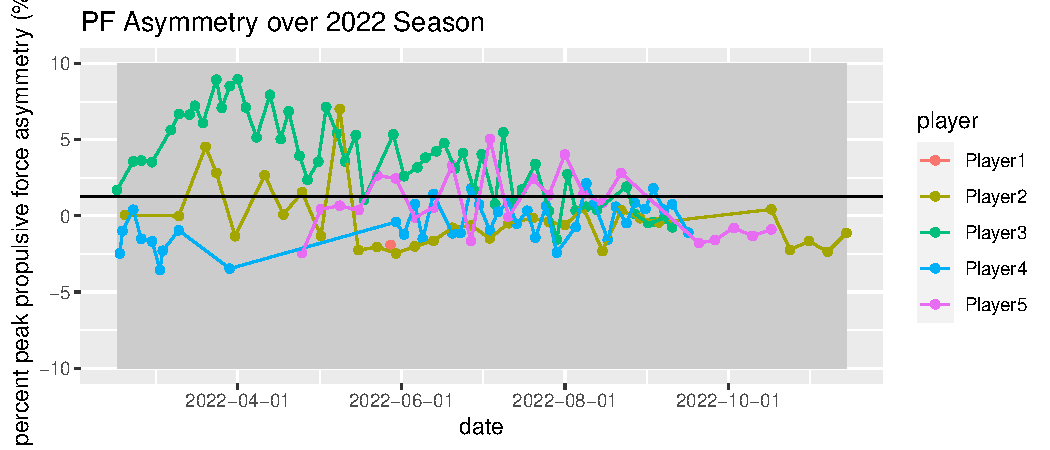
\includegraphics{report_code_files/figure-latex/imbalance-1.pdf}
\caption{Propulsive Force Imbalance over 2022 season. Black line is mean
and ribbon is =/-2 sd}
\end{figure}

\hypertarget{workload}{%
\paragraph{Workload}\label{workload}}

When comparing each player to themselves over the season, overall there
was only one player that had a jump outside of their 2 sd ribbon (Figure
3). Only Player 2 had a jump in April that was outside of the ribbon,
which is more than likely from a steady decline in their PI. This could
be a sign of steady fatigue throughout the year and possibly something
to pay attention to with this player for next season. Players 3 and 4
had a steady increases after the All-Star break, which shows that there
were either strategies changed after the break, or the training
adaptations were able to take effect with the time off. Player 5 started
low when they began jumPIng in May, but was able to maintain themselves
throughout the year. What is interesting with Player 5 is the drop in
weight from September to October, also corresponds with their drop in PI
so this drop in weight and PI may have been from an increased workload.
Player 1 only has one day of jumps, they are excluded from this section.

\begin{figure}
\centering
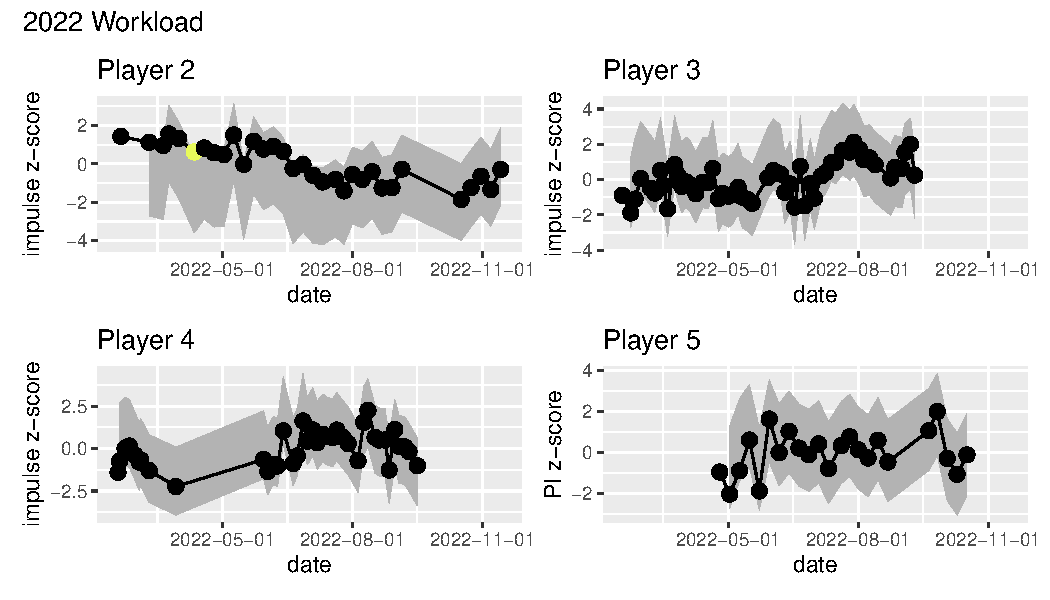
\includegraphics{report_code_files/figure-latex/workload-1.pdf}
\caption{Workload over the 2022 season by player. Ribbon is 28-day
rolling mean +/- 2 sd.}
\end{figure}

\hypertarget{sources}{%
\subsubsection{Sources}\label{sources}}

Benjanuvatra N, Lay BS, Alderson JA, Blanksby BA. Comparison of ground
reaction force asymmetry in one- and two-legged countermovement jumps. J
Strength Cond Res. 2013 Oct;27(10):2700-7. doi:
10.1519/JSC.0b013e318280d28e. PMID: 23287834.

Cone, Simon, ``Lower Limb Force Asymmetries during Landing and JumPIng
Exercises'' (2020). Master's Theses. 5141

Hewit, Jennifer MSc, CSCS1; Cronin, John PhD1,2; Hume, Patria PhD1.
Multidirectional Leg Asymmetry Assessment in Sport. Strength and
Conditioning Journal: February 2012 - Volume 34 - Issue 1 - p 82-86 doi:
10.1519/SSC.0b013e31823e83db

Sands, W. A., Kavanaugh, A. A., Murray, S. R., McNeal, J. R., \& Jemni,
M. (2017). Modern techniques and technologies applied to training and
performance monitoring. International Journal of Sports Physiology and
Performance, 12(Suppl 2), 63--72.
\url{https://doi.org/10.1123/ijspp.2016-0405}

\end{document}
